To compute self energies, we follow \cite{Bojak:2000eu}.
It is
\begin{align}
\{\gamma_\mu,\gamma_\nu\} &= 2g_{\mu\nu}\\
\gamma_\mu\gamma^\mu &= g_\mu^\mu = n \\
\gamma_\mu\gamma_\nu\gamma^\mu &= (2-n)\gamma_\nu
\end{align}
\begin{figure}[ht!]
	\begin{subfigure}[t]{.4\textwidth}
		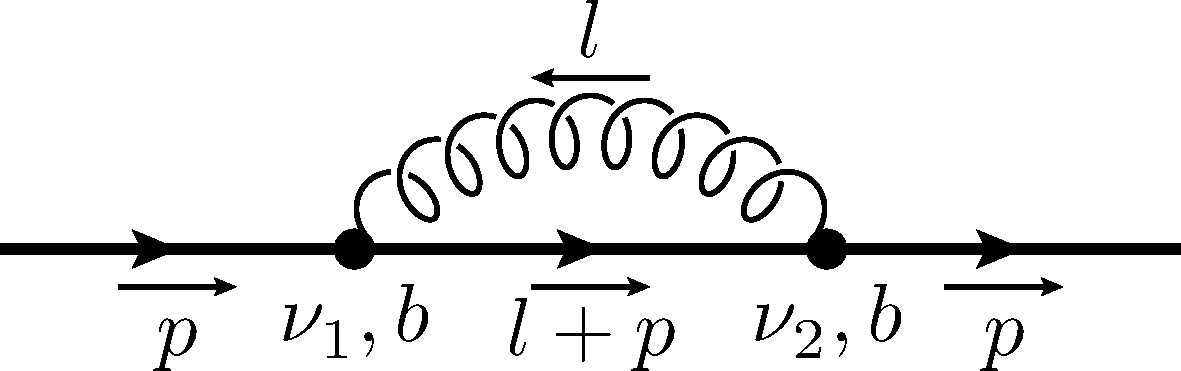
\includegraphics[width=\textwidth]{pyfeyn/nlo-v-seq}
		\caption{$-i\Sigma(p)$}
	\end{subfigure}\hspace{.15\textwidth}%
	\begin{subfigure}[t]{.4\textwidth}
		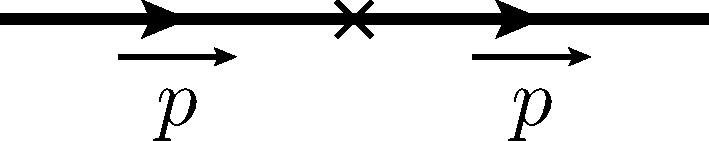
\includegraphics[width=\textwidth]{pyfeyn/nlo-v-seqc}
		\caption{$-i\Sigma_C(p)$}
	\end{subfigure}
	\caption{NLO contributions by quark self energy}\label{fig:FeynNLOvseq}
\end{figure}
\begin{align}
-i\Sigma(p) &= \mu_R^{4-n}\!\!\int\!\!\frac{d^nl}{(2\pi)^n}(igT_b \gamma_{\nu_1})\frac{i(\slashed{l}+\slashed{p}+m)}{(l+p)^2-m^2}(igT_b \gamma_{\nu_2})\frac{-ig^{\nu_1,\nu_2}}{l^2}\\
 &=-\mu_R^{4-n}g^2C_F\!\!\int\!\!\frac{d^nl}{(2\pi)^n}\frac{2m+(2-n)\slashed{p}+(2-n)\slashed{l}}{l^2((l+p)^2-m^2)}\\
 &=-g^2C_F\left(\left(2m+(2-n)\slashed{p}\right)B_0(p^2,0,m^2)+(2-n)B_1(p^2,0,m^2)\right)\\
 &=-g^2C_F\left(B_0(p^2,0,m^2)\left(n\cdot m+(2-n)\slashed{p}\frac{p^2+m^2}{2p^2}\right)-(2-n)\slashed{p}\frac 1{2p^2}A_0(m^2)\right)
\end{align}
Using \cite{Bojak:2000eu} we find
\begin{align}
C_\epsilon &= \frac 1 {16\pi^2}\exp\left(\left(\gamma_E-\log(4\pi)\right)\frac{\epsilon} 2\right)\left(m^2/\mu^2\right)^{\epsilon/2}\\
A_0(m^2) &=iC_\epsilon\left(-\frac 2 {\epsilon}+1\right)\\
B_0(p^2,0,m^2) &=iC_\epsilon\left(-\frac 2{\epsilon}+2+\frac{m^2-p^2}{p^2}\ln\left(\frac{m^2-p^2}{m^2}\right)\right)
\end{align}
\begin{align}
\Rightarrow-i\Sigma(p) &= -ig^2C_FC_\epsilon\left[\frac{2\slashed{p}-8m}{\epsilon}+2m\left(3-2\left(1-\frac{m^2}{p^2}\right)\ln\left(1-\frac{p^2}{m^2}\right)\right)\right.\nonumber\\
 &\hspace{90pt}\left.-\slashed{p}\left(1+\frac{m^2}{p^2}\right)\left(1-\left(1-\frac{m^2}{p^2}\right)\ln\left(1-\frac{p^2}{m^2}\right)\right)\right]\\
 &\EqualClaim -i(A m + B(\slashed p - m))
\end{align}
\begin{align}
\Rightarrow A &= \frac 1 m \left.\Sigma(p)\right|_{\slashed{p}=m} \\
 &= -g^2C_F C_\epsilon\left(\frac 6 \epsilon -5 +\frac{m^2}{p^2}+\left(3-4\frac{m^2}{p^2}+\frac{m^4}{p^4}\right)\ln\left(1-\frac{p^2}{m^2}\right)\right)\\
\Rightarrow B &= \frac 1 m \left.\DeriveF{\slashed{p}}{\Sigma(p)}\right|_{\slashed{p}=m} \\
 &= \frac{g^2}{16\pi^2}C_F \left(\frac 2 {\hat\epsilon_m} -1-\frac{m^2}{p^2}+\left(1-\frac{m^4}{p^4}\right)\ln\left(1-\frac{p^2}{m^2}\right)\right)
\end{align}

Counterterm:
\begin{align}
-i\Sigma_C(p) &=i((Z_2-1)\slashed{p}-(Z_2 Z_m -1) m)\\
 &= i((Z_2-1)(\slashed p - m) - (Z_m-1)m) + O(\alpha_S^2)
\end{align}

Use on-shell renormalisation:
\begin{align}
0 &\EqualClaim \left.\left(-i\Sigma(p)-i\Sigma_C(p)\right)\right|_{\slashed{p}=m}\\
 &= i\left.\left(((Z_m-1)+A)m+(B-(Z_2-1))(\slashed p - m)\right)\right|_{\slashed{p}=m} \\
\Rightarrow (Z_m-1) &= \left.-A\right|_{\slashed{p}=m}\\
 &= \frac{g^2}{16\pi^2}C_F \left(\frac 6 {\hat \epsilon_m} -4\right)
\end{align}

We also choose
\begin{align}
Z_2-1 &= \frac{g^2}{16\pi^2}C_F \frac 2 {\hat \epsilon_m}\\
Z_{1f} &= Z_2 + \frac{g^2}{16\pi^2}C_A\frac 2 {\hat \epsilon}
\end{align}
